\documentclass[11pt]{scrartcl}
\usepackage{tikz}

\begin{document}
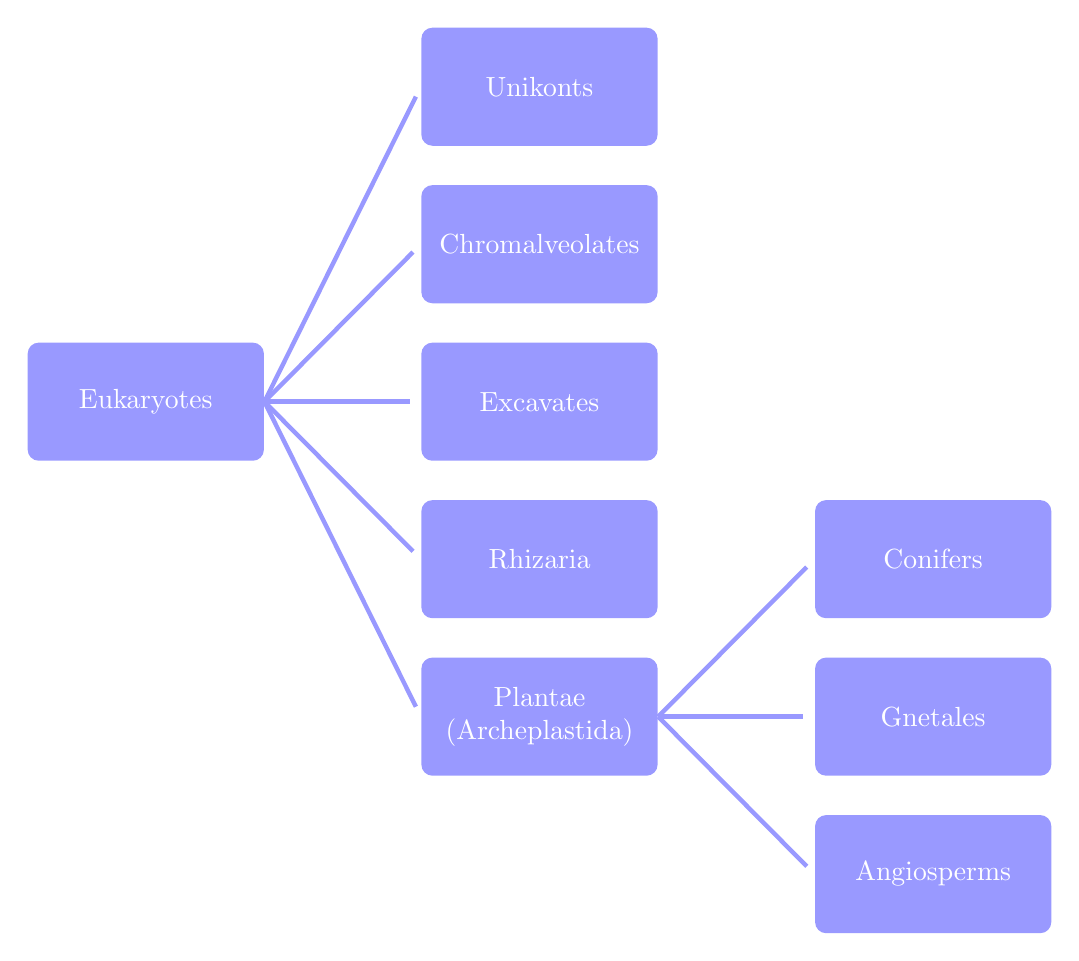
\begin{tikzpicture}[every node/.style = {shape          = rectangle,
                                         rounded corners,
                                         fill           = blue!40!white,
                                         minimum width  = 3cm,
                                         minimum height = 1.5cm,
                                         align          = center,
                                         text           = white},
                   blue edge/.style  = { -,
                                         ultra thick,
                                         blue!40!white,
                                         shorten >= 4pt}]

% the nodes : possible  \newcommand*\dx{5} \newcommand*\dy{2}
\node(0;0) at (0,0) {Eukaryotes};
  \node(1;2)  at (5, 4) {Unikonts};   
  \node(1;1)  at (5, 2) {Chromalveolates}; 
  \node(1;0)  at (5, 0) {Excavates}; 
  \node(1;-1) at (5,-2) {Rhizaria}; 
  \node(1;-2) at (5,-4) {Plantae\\
                   (Archeplastida)};
     \node(2;1)  at (10,-2) {Conifers};
     \node(2;0)  at (10,-4) {Gnetales};
     \node(2;-1) at (10,-6) {Angiosperms};

% edges 
\foreach \j in {-2,...,2}
  { \draw[blue edge] (0;0.east) -- (1;\j.west); }
\foreach \j in {-1,...,1}
  { \draw[blue edge] (1;-2.east) -- (2;\j.west);}                  
\end{tikzpicture}
\end{document} 